\chapter{Neural Networks and Fourier Neural Operators}\label{ch:FNO+NN}
So far, we have studied numerical methods for solving partial differential equations (PDEs).
The finite volume method (FVM), along with other numerical solvers such as the finite difference method (FDM) and finite element method (FEM), solves PDEs by discretizing the domain into a grid.
A finer grid improves the accuracy of the solution but also increases the computational cost, creating a trade-off between accuracy and efficiency.
Complex PDEs often require a fine grid to accurately capture the solution, which can be computationally expensive.
This motivates the use of data-driven methods, which have shown great potential in handling large data sets and learning complex patterns in the data.

In this chapter, we introduce the use of data-driven methods for solving PDEs.
We will introduce the concepts of convolutional neural networks (CNNs) and Fourier neural operators (FNOs).
A basic understanding of neural networks is assumed, for example through courses in machine learning or deep learning.
Both methods rely solely on data, rather than the PDE itself, which is particularly useful when the governing PDE is unknown.
The hope of data-driven methods is that they are able to reduce computational costs while maintaining high accuracy by learning the underlying dynamics of the solution.
This could also help making predictions for the solution of the shallow water equations (SWE) outside the training data.


\section{Convolutional Neural Networks}\label{sec:CNN}
Convolutional neural networks (CNNs) are a specialized class of artificial neural networks (ANNs) designed to process and analyze data with a grid-like topology, such as images or time-series data represented by 2D grids.
CNNs excel at extracting spatial featues from data through the use of convolutional layers, which apply learnable filters to detect patterns such as edges, shapes or textures.
These layers are typically followed by pooling layers for dimensionality reduction and fully connected layers for classification or regression tasks.
A key advantage of CNNs is their ability to reduce the number of parameters compared to fully connected neural networks by sharing weights across spatial regions, making them computationally efficient and less prone to overfitting when working with large inputs.
Although CNNs are traditionally used for image recognition tasks, their architecture is adaptable for time-series analysis, especially when the data is structured spatially or sequentially~\cite{chollet2017comprehensive}.

In this project, CNNs are used to solve the SWE, by training on the solution data generated by the FVM solver.
We aim to learn the underlying dynamics of the system by training the CNN on sequences of input-output pairs, where the input $\mathbf{x}(t)$ is the state of the system at time $t$ and the output is the state at time $t + \Delta t$, denoted by $\mathbf{x}(t + \Delta t)$.
More specific, this means that the CNN model is trained on input-output pairs of sequences of data, with a sequence length of $n$, illustrated in the vectors below:
\begin{align*}
    \begin{bmatrix}
        x_i \\ x_{i+1} \\ \vdots \\ x_{i+n-1}
    \end{bmatrix}
    \to
    \begin{bmatrix}
        x_{i+1} \\ x_{i+2} \\ \vdots \\ x_{i+n}
    \end{bmatrix},
    \text{ for} \quad i = 0, 1, \ldots, N-n,
\end{align*}
where $x_i$ is the state of the system at time $i$.
The input-output pairs are designed to train the CNN to predict the system's state at the next time step, based on the current state and the $n-1$ previous states.
%We also want to predict the solution of the SWE at future time steps, which is why we use sequences of input data.
Hence, the network is trained to construct a flow map, which is a mapping from the current state to the next state.
The flow map $\Phi: \mathbb{R}^n \rightarrow \mathbb{R}^n$ is defined such that, for all $x \in X$, where $X$ is the solution space, and all $t \in \mathbb{R}$:
\begin{align*}
    \Phi(x_0) =  x(t),
\end{align*}
where $x(t)$ is the solution of the PDEs with initial condition $x(0) = x_0$.
The flow map satisfies
\begin{align*}
    \Phi(\Phi (x, t), s) = \Phi(x, s + t),
\end{align*}
A CNN can approximate the flow map $\Phi$ by training on data that pairs a state $\mathbf{x}(t)$ with its state at later times $\mathbf{x}(t + \Delta t)$.
The goal is to learn the mapping:
\begin{align*}
    x_{i+1} = \Phi_{CNN} (x_i), 
\end{align*}
where $\Phi_{CNN}$ is the CNNS' approximation of the flow map.
The network process a sequence of input data to predict the corresponding output data.
The CNN's output is the solution at the next time step, effectively learning the dynamics of the SWE through the time-series data.
This setup allows the model to capture both spatial and temporal dependencies in the data, leveraging the CNN's ability to learn localized featires while processing sequential information.
An advantage of CNNs is their efficiency.
By processing data in parallel using convolutional layers, the CNN efficiently handles large datasets without requiring excessive computational resources.
Another strengt is their adaptability. The model's ability to learn from sequential data makes it adaptable for time-series predictions in dynamic systems like the shallow water equations.
However, a drawback is the challenge of data representation.
Representing time-series data as sequences may require preprocessing, which can introduce complexity or a potential loss of information.
%We will train, test and evaluate the performance of several CNN models in \autoref{ch:data-driven-results}.
The results of the CNN models will be presented in \autoref{ch:data-driven-results}.

\section{Fourier Neural Operators}
In this section, we introduce the concept of Fourier Neural Operators (FNOs), based on the method and theory presented in~\cite{FNO_2021}.
FNOs are distinctive since, unlike classical neural networks that primarily learn mappings between finite-dimensional spaces, they approximate mappings between infinite-dimensional function spaces.
The goal of an FNO is to learn a mapping between two infinite-dimensional spaces from a finite collection of input-output pairs.
Consider the operator $G: A \to U$, which maps functions from an infinite-dimensional function space $A$ to another infinite-dimensional function space $U$.
Out objective is to approximate the exact operator $G$ by constructing the map
\begin{align}\label{eq:FNO_map}
    G_{\theta}: A \mapsto U, \quad \theta \in \Theta,
\end{align} 
where $\Theta$ is a finite-dimensional parameter space.
Let $a \in A$ and $u \in U$ represent the input and output functions, respectively.
We assume access to data in the form of pointwise evaluations of these functions, i.e., we have access to the observations ${\{a_j, u_j \}}_{j=0}^{N-1}$, in a domain $D \subset \mathbb{R}$, which is a bounded open set.
The observations are time shifted, meaning $u_j = G(a_j)$, where $G$ is the true operator, and $u_j = a_{j+1}$ for all $j = 0, 1, \ldots, N-1$.
Thus, the goal is to approximate the mapping $a_j \mapsto u_j$ for all $j = 0, 1, \ldots, N-1$.

The process begins with the input layer $P$, typically a shallow fully connected neural network, which generates $v_0(x) = P(a(x))$.
The FNO is an iteraive neural operator, applying several updates to compute intermediate representations $v_1, v_2, \ldots, v_T$.
In the context of this project, we have that $a(x) = v_t(x)$ and $u(x) = v_{t+1}(x)$.
An update $v_t \mapsto v_{t+1}$ is defined as
\begin{align}
    v_{t+1}(x) := \sigma \left( W v_t(x) + \left( \mathcal{K}(a;\phi)v_t \right) (x) \right), \quad \forall x \in D,
\end{align}
where $W: \mathbb{R} \to \mathbb{R}$ is a linear transformation, $\sigma: \mathbb{R} \to \mathbb{R}$ is a non-linear activation function, and $\mathcal{K}(a;\phi)$ is a kernel function parameterized by $\phi$.
The final update $v_T(x)$ is transformed by the output layer $Q$ to produce the output $u(x) = Q(v_T(x))$, ensuring the correct output dimensions.
Similar to the CNN approach, state pairs ${\{v_t, v_{t+1}\}}_{j=0}^N$ are collected for training the flow map, represented by $G_{\theta}$.
Feeding this data into the FNO model enables it to learn the flow map for the system.

There are various types of operators, but the core of the Fourier neural operator lies in its kernel function $\mathcal{K}$.
We define the Fourier integral operator $\mathcal{K}$ as 
\begin{align}
    \left( \mathcal{K}(\phi)v_t \right) (x) := \mathcal{F}^{-1} \left( R_{\phi} \cdot (\mathcal{F}v_t ) \right)(x), \quad \forall x \in D,
\end{align}
where $\mathcal{F}$ is the Fourier transform, $\mathcal{F}^{-1}$ is the inverse Fourier transform, and $R$ is the linear transformation applied on the lower Fourier modes. 
Recall that the Fourier transform of a function $f(t)$ is defined as~\cite{Fourier_Transform}:
\begin{align}
    \mathcal{F} (f(t)) = \hat{f}(s) = \int_{-\infty}^{\infty} e^{ -2 \pi ist} f(t) dt,
\end{align}
and correspondingly the inverse Fourier transform of a function is
\begin{align*}
    \mathcal{F}^{-1} (\hat{f}(s)) = f(t) = \int_{-\infty}^{\infty}  e^{2 \pi ist} \hat{f}(s) ds.
\end{align*}
By transforming the data into the Fourier domain, FNOs can take advantage of the periodicity and smoothness properties of the Fourier basis, which simplifies the learning process for functions defined over continuous domains.
%This approach leverages the fact that differentiation with respect to time is equivalent to multiplication in the Fourier domain, not to be interchanged with the convolution theorem. CITE.
The network architechture for the FNO model is illustrated in \autoref{fig:fourier_neural_network}.
\begin{figure}[H]
    \centering
    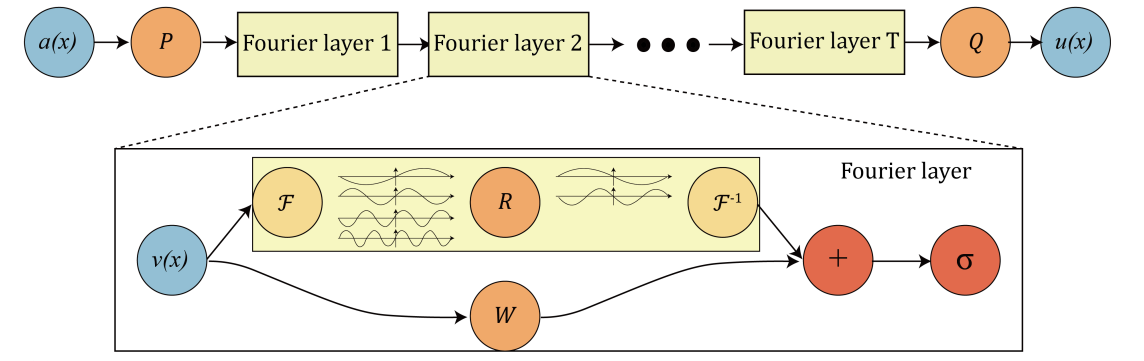
\includegraphics[width=0.7\textwidth]{C:/Users/Matteo/Shallow-Water-Equations/figs/fourier_neural_network.png}
    \caption{An overview of the network architecture with several Fourier layers. Illustration from~\cite{FNO_2021}.\\
            Top: Overall structure with input function $a$, input layer $P$, several Fourier layers, output layer $Q$ and output function $u$.\\
            Bottom: A Fourier layer consists of two parallel paths. Top is a Fourier transformation $\mathcal{F}$, a linear transformation $R$ and an inverse Fourier transformation $\mathcal{F}^{-1}$.
            The bottom path consists of a linear transformation $W$. The parts meet and undertake an activation function $\sigma$.}\label{fig:fourier_neural_network}
\end{figure}
From the top in \autoref{fig:fourier_neural_network} we see that the network consists of an input function $a(x)$, an input layer $P$, several Fourier layers, an output layer $Q$ and some output function $u(x)$.
In the bottom of \autoref{fig:fourier_neural_network} we see the structure of a Fourier layer, which consists of two parallel paths.
In the top path, the data undergoes a Fourier transform $\mathcal{F}$, decomposing it into a sum of Fourier basis functions (sines and cosines) with varying frequencies, amplitudes and phases.
A linear transformation $R$ it then applied to filter out the higher Fourier modes, as illustrated in the figure, where high-frequency components are removed.
When implementing the model, we choose the number of Fourier modes to retain, depending on how much information we want to preserve.
Retaining more modes keeps more information, but may also introduce more noise and oscillations.
After filtering, the inverse Fourier transform $\mathcal{F}^{-1}$ is applied to reconstruct the data in its original form.
The bottom path involves a linear transformation $W$, and the two paths merge before applying a non-linear activation function $\sigma$.

A key advantage of FNOs is their ability to learn mappings between function spaces, making them independent of any specific grid or mesh.
This allows them to transfer solutions across different grids, a capability known as zero-shot super-resolution.
For instance, the learned operator can generalize from a coarse grid to a fine grid without retraining.
This feature significantly reduces the computational cost associated with fine-grid simulations.
In \autoref{ch:data-driven-results}, we will evaluate the performance of the implemented FNO model in this context, testing its ability to maintain high accuracy when making predictions on finer grids.

\subsection*{Multistep prediction}
Current literatur highlights the strong performance of FNOs in long-term predictions.
One potential application of the FNO model is predicting the solution of the SWE at multiple future time steps.
We aim to develop a multi-step prediction model capable of forecasting a specified number of time steps ahead.
In its original form, the FNO is designed to predict one time step ahead.
However, for many practical applications, multi-step predictions are more useful.
The first, naive approach to achieve this is to use the model iteratively: predicting the solution at the next time step, then using that prediction as input to predict the solution at the next time step, and so on.
However, as one can imagine this approach quite fast lead to inaccurate predictions, as errors accumulate over time.

To improve the accuracy of multi-step predictions, we train the model on sequences of input data, where the input data consists of several previous time steps.
The sequential data is formatted similarly to that used in the CNN, with input sequences of length $n$.
The model is trained to predict the output state based on this sequence of previous time steps.
We will conduct experiments to determine the optimal sequence length for our model.
That is, we train the model on input-output pairs of sequences, each with a sequence length of $n$, as illustrated in the vectors below:
\begin{align*}
    \begin{bmatrix}
        v_{t-n} \\ v_{t-n+1} \\ \vdots \\ v_{t-1} \\ v_t
    \end{bmatrix}
    \to
    \begin{bmatrix}
        v_{t-n+1} \\ v_{t-n+2} \\ \vdots \\ v_{t} \\ v_{t+1}
    \end{bmatrix},
    \text{ for} \quad t = 0, 1, \ldots, N-n.
\end{align*}
Training the model on sequences of input data allows it to learn the dynamics of the system over time, capturing both short-term and long-term dependencies in the data.
It also makes the model more accurate by providing more context for making predictions, ensuring that recent predictions do not disproportionately influence future predictions.
When making multi-step predictions, the model's output is added to the input as the newest data point, replacing the oldest data.
This process is repeated until predictions for the desired number of future time steps are made.
The process is illustrated in \autoref{fig:multistep_pred_flowchart}.
\begin{figure}[H]
    \centering
    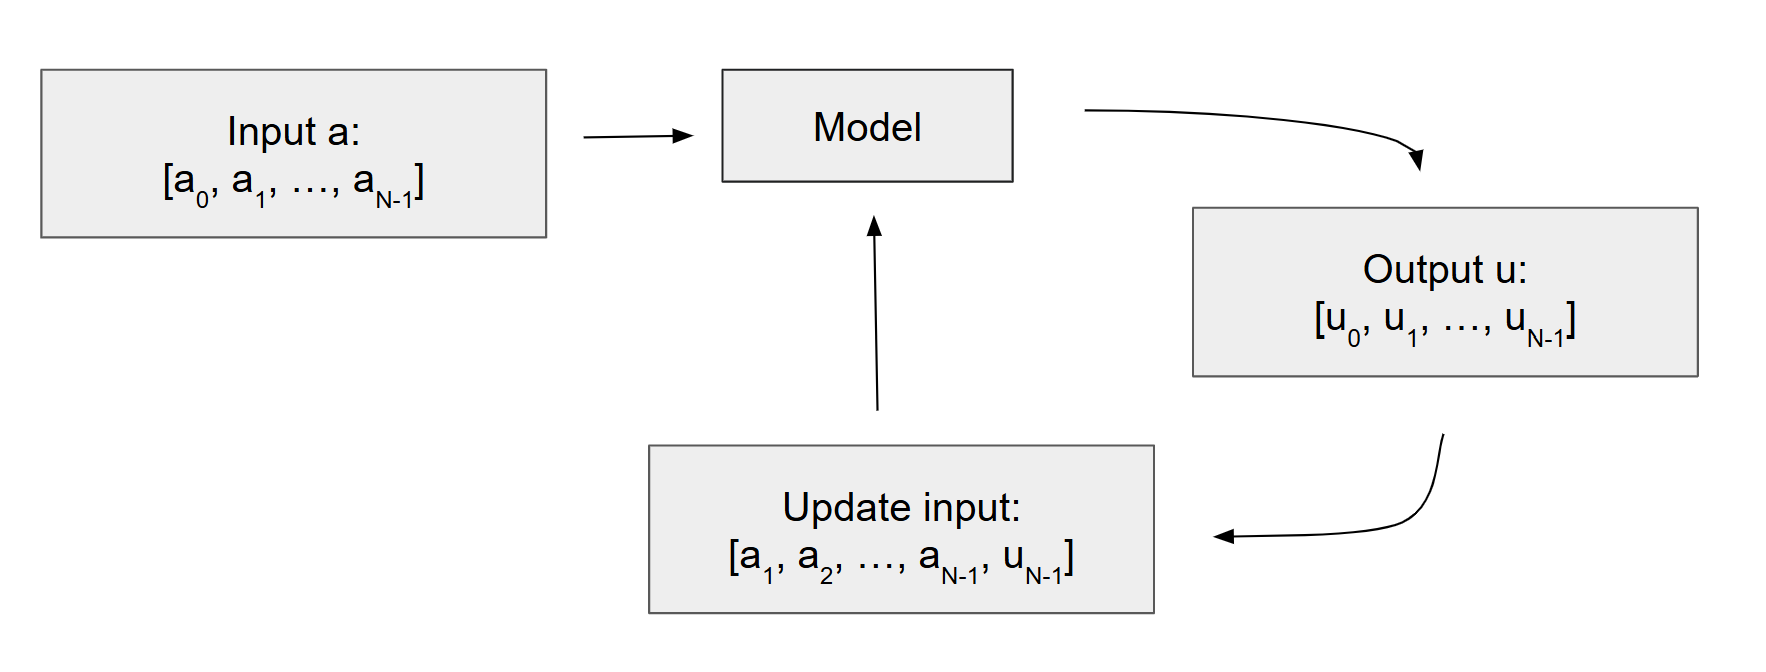
\includegraphics[width=0.7\textwidth]{C:/Users/Matteo/Shallow-Water-Equations/figs/multistep_pred_flowchart.png}
    \caption{Flowchart of the multi-step prediction process.}\label{fig:multistep_pred_flowchart}
\end{figure}
In \autoref{fig:multistep_pred_flowchart}, we present the flowchart of the multi-step prediction process.
Starting with the input data $a$, the model makes predictions $u$, which are then used to update the input data for the next predictions.
This process is applied to both the CNN and FNO models.
The results of the multi-step prediction model will be presented in \autoref{ch:data-driven-results}.
%Another issue we are facing in this project is non-linearities.
%Whereas, neural operators approximate non-linear operators, by combining linear functions and non-linear activation functions with global integral operators. 